\section{New approximate pattern mathing algorithms}
\label{section:our}

In the section we present two algorithms for approximate pattern mathing that heavily based on semi-local sequence alignment and its underlying algebraic structure.
The presented algorithms also support length constraints on the result (on detected clones).

\subsection{First algorithm}
The first algorithm~\ref{alg:appximateMatchingGreedy} implements an idea of the greedy choice of the most suitable clone on each step, i.e. it looks for the most similar substring with length in interval $[l,\ r]$ each time for some predefined constants $l$ and $r$.
In other words, it constructs a non-intersected set $\Tau$ of clones of pattern $p$ in text $t$ such that on each step it adds $\tau_k$ to $\Tau$ iff $\tau_k$ has the highest similarity score with $p$ in the rest of the text and its length satisies the length constraint, i.e. $l \leq |\tau_k| \leq r$.
%% The first algorithm~\ref{alg:appximateMatchingGreedy} refers to following constraint.
%% There should be found all non-intersected clones $\tau_{k}$ of pattern $p$ from text $t$ that has the highest similarity score on the uncovered part of the text $t$ and $l \geq |\tau_{k}| \geq r$  i.e algorithm should perform greedy choice at each step with length constraint on $\tau_{k}$.
%% This is a more intuitive approach i.e like looking for the most similar substring every time with length at least $l$ and at most $r$.
%% Formally:\todo{check l and r}
%% \begin{equation}
%%    \Tau = \bigcup_{k} \tau_k = \bigcup_k \argmax_{l,r \in (t \cap (\cup_{j=1}^{i-1} \tau_{j}),l<r, l \leq |t_{l,r}| \leq r ,t_{l,r} \cap (\cup_{j=1}^{i-1} \tau_{j}) = \emptyset } sa(t_{l,r}, p)
%% \end{equation}

The algorithm proceeds as follows.

First, the semi-local sa problem is solved for given pattern $p$ and text $t$ (line 1).
Then, the solution for the string-substring subproblem is queried from it (lines 2--3).
Further, the diagonal slice of width $r-l$ which corresponds to scores of substrings of size in $[l,\ r]$ is cropped to get a partial Monge matrix (line 4) (see Fig.~\ref{figures:M1}).
Next, using Theorem~\ref{partialTheorem} a \emph{rmq2D} data structure is constructed (lines 5--6) which make it possible to perform range minimum queries.
%% \todo{Upon partial matrix $M_{partial}$, the full Monge Matrix $M$ is built to build \emph{rmq2D} data structure  for performing range minimum queries on $M$ by Theorem \ref{partialTheorem}.}

\begin{figure}[!t]
  \centering
    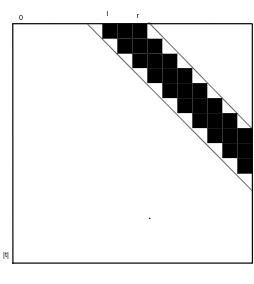
\includegraphics[width=0.4\columnwidth]{figures/M1.png}
    \caption{The diagonal in matrix represent a set of substrings of text $t$ that have size in $[l,r]$ interval.}\label{figures:M1}
\end{figure}

Then, algorithm calls recursive subroutine $greedy$ (algorithm \ref{alg:rec}).
The $greedy$ routine performs greedy choice of $\tau_{k}$ with maximal alignment within a continious uncovered part of the text $t_{i,j}$ with length boundaries for $\tau_{k}$ in $[l,\ r]$ where $t_{i,j}$ denotes a substing of text $t$ starting at $i$-th element and ending at $j$-th element.
More precisely, it refers to searching maximum value with corresponding position (row and column) in matrix $M$ within $t_{i,j}$.
The search is performed via range queries.
When detected $interval$ has alignment score less then threshold it means that no clones of pattern $p$ are presented in this part of text $t_{i,j}$, and further processing should be skipped.
Otherwise, the founded clone $\tau_k$ is added to the final result and the current part of the text splits into two smaller parts and processed recursively in the same way.

Finally, the algorithm outputs a set of the non-intersected intervals of clones of pattern $p$ in text $t$.


\begin{algorithm}[!t]
\caption{Greedy subroutine}
\label{alg:rec}
Input: $rmq2D$--- range maximum query data structure for performing range queries on Monge matrix $M$, $h$ --- threshold value, $i,j$ --- start and end positions of current text $t_{i,j}$, $l,r$--- length boundaries for detected intervals \\
Output: Set of non-intersected intervals from $t_{i,j}$\\
Pseudocode:\\
$greedy(rmq2D,h, i, j, t_{i,j},l,r ):$

\begin{algorithmic}[1]
\STATE{$interval = rmq2D.query(i,j,i,j)$}
\STATE{$result = \emptyset$}
\IF{ $interval.score < h $}
\RETURN $result$
\ENDIF
\IF{ $interval.i - i \geq l $}
\STATE{$cl = greedy(rmq2D,h,i,interval.i,t_{i,interval.i},l,r)$}
\STATE{$result.add(cl)$}
\ENDIF
\IF{$j - interval.j \geq l$}
\STATE{$cl = greedy(rmq2D,h,j,interval.j,t_{j,interval.j},l,r)$}
\STATE{$result.add(cl)$}
\ENDIF
\RETURN $result$
\end{algorithmic}
\end{algorithm}


\begin{algorithm}[!t]
\caption{GREEDY-PATTERN BASED NEAR DUPLICATE
SEARCH ALGORITHM}
\label{alg:appximateMatchingGreedy}
Input: pattern $p$ and text $t$, threshold value $h$\\
Output: Set of non-intersected clones of pattern $p$ in text $t$\\
Pseudocode:\\
$GreedyMathing(M,h,t)$
\begin{algorithmic}[1]
\STATE{$sa = semilocalsa(a,b)$}
\COMMENT{1st phase}
\STATE{$H = sa.getAssociatedMatrix()$}
\STATE{$H^{str-sub} = H.stringSubstringMatrix()$}
\STATE{$M_{partial} = -getPartialMatrix(H^{str-sub},l,r)$}
\COMMENT{2nd phase}
\STATE{$M = builtMongeMatrix(M_{partial})$}

\STATE{$rmq2D = buildRMQStructure(M) $}
\STATE{$result = greedy(rmq2D,h,0,|t|,t,l,r)$}
\COMMENT{3rd phase}
\RETURN $result$
\end{algorithmic}
\end{algorithm}


\begin{theorem}
Algorithm~\ref{alg:appximateMatchingGreedy} runs in $O(max(|t||p|,\frac{|t| \log^2 |t|}{\log \log |t|} ))$ time and $O(|t|)$ space when $|p|<|t|$ where $p$ is pattern, $t$ is text, and $v=O(1)$ is denominator of normalized mismatch score for semi-local sequence alignment $w_{normalized} = (1,\frac{\mu}{v},0)$.
\end{theorem}
\begin{proof}
Note that $|p|<|t|$ and $v=O(1)$.
For simplicity let $v=1$ (same true for other $v=O(1)$).

\emph{First phase}. 
Since $v=1$ we need to solve semi-local lcs problem.
It could be solved implicitly via algorithm from~\cite{tiskin2008semi} in $O(|t| * |p|)$ with $O(|t|)$ additional space when $|p|<|t|$.
Note, we are only interested in string-substring submatrix $H^{str-sub}_{p,t}$ of size $|t| \times |t|$.
By Theorem~\ref{decomposition} we build data structure of size $O(|t|)$ in $O(|t|\sqrt{\log(|t|))}$ time from associated permutation matrix with $H^{str-sub}_{p,t}$ anti-Monge matrix~\cite{chan2010counting}.
The data structure performs orthogonal range queries in $O(\frac{\log (|t|)}{\log \log (|t|)})$ time.
%% \todo{Upon} associated permutation matrix with $H^{str-sub}_{p,t}$ anti-Monge matrix ( Theorem \ref{decomposition}) we build data structure of size $O(|t|)$ in $O(|t|\sqrt{\log(|t|))}$ time to perform orthogonal range queries in $O(\frac{\log (|t|)}{\log \log (|t|)})$ time.
Thus, the overall time and space complexity of first phase 
is $max(O(|t|*\sqrt{\log(|t|))},\ O(|p|*|t|))$ and
$O(|t|)$ respectively.

\emph{Second phase}.
In string-substring matrix $H^{str-sub}_{p,t}$ we are only interested in diagonal of length $r-l$ that refers to all substrings of text $t$ with length in $[l:r]$ interval. 
Hence, we inverce matrix  $H^{str-sub}_{p,t}$ and pick out the diagonal of interest, resulting in partial Monge matrix $M_{partial}$.
%% If we apply to  $H^{str-sub}_{p,t}$ inverse operation and cut this diagonal we will have partial Monge matrix $M_{partial}$.
Then we apply theorem  \ref{partialTheorem} to build 
\emph{rmq2D} data structure to perform minimum range queries.
Note, access to the element in $M_{partial}$ can be performed in non-constant and it returns not the only element itself but also the associated indices.
Hence, the data structure of size $O(|t|)$ can be built in $O(|t| \log |t|)* O(\frac{\log (|t|)}{\log \log (|t|)}) = O(\frac{|t|\log^2 |t|}{\log \log (|t|)}) $ time to perform range minimum queries in $O(\log \log (|t|))*O(\frac{\log (|t|)}{\log \log (|t|)}) = O(\log |t|)$ time.
Thus, overall time and space complexity of second phase are $O(|t| \log^2 |t|)$ and $O(|t|)$ respectively.

\emph{Third phase}.
To analyze the third phase we need to look at the recursive algorithm~\ref{alg:rec}.
Note, at the worst case we will have $O(|t|)$ nodes while proceeded recursion since at the worst case on each node we will detect interval of size $1$.
There will be at most $t$ such non-intersecting intervals.
Thus, the total amount of calls to $query$ operation will be at most $O(|t|)$.
The query operation requires time $O(\log |t|)$ as shown in the previous phase.
Hence, the total running time and space complexity of third phase are $O(|t| |\log t|)$ and $O(|t|)$  

Thus, overall algorithm running time and space complexity are as claimed when $v=O(1)$ and $|p|<|t|$.
\end{proof}

\subsection{Second algorithm}
The second algorithm \ref{alg:appximateMatchingMax} uses a less sophisticated approach and finds fewer duplicates of pattern $p$.
It is similar to the previous one but uses simplier approach instead of the $greedy$ subrutine.

\paragraph{Algorithm description}

The first phase as in algorithm~\ref{alg:appximateMatchingGreedy}.
On the second phase we use Lemma~\ref{lemma} to implicitly fill elements of partial Monge matrix to get the Monge matrix $M$.
Then we solve the following problem (Line 6).
For each prefix of text $t$ we find the suffix that has the highest similarity score with pattern $p$:
$$ a[j] = \max _{i \in 0 ..j} sa(p,t[i,j]), j \in 0..|t|.$$

Further, we remove suffixes whose similarity score is below the given threshold $h$ (line 4).
Then remaining suffixes are sorted in descending order (line 5) and an interval tree~\cite{pal2009interval} is built upon them (lines 9--14).
The building process consists of checking that current substring $candidate$ not intersected with already added substrings to the $tree$ and adding it in case of success.
Finally, algorithm outputs a set of non-intersected substrings (clones) of pattern $p$ in text $t$.

\begin{algorithm}[!t]
\caption{Greedy approximate}
\label{alg:appximateMatchingMax}
Input: pattern $p$, text $t$, threshold value $h$\\
Output: Set of non-intersected clones of pattern $p$ in text $t$\\
Pseudocode:
\begin{algorithmic}[1]

\STATE{$sa = semilocalsa(p,t)$}
\COMMENT{1st phase}
\STATE{$H = sa.getAssociatedMatrix()$}
\STATE{$H^{str-sub} = H.stringSubstringMatrix()$}
\STATE{$M_{partial} = -getPartialMatrix(H^{str-sub},l,r)$}
\STATE{$M = fillToMongeMatrix(M_{partial})$ }
\COMMENT{2nd phase}
\STATE{$colmax = smawk(M) $}
\STATE{$colmax.filter(it.score >= h$)}
\STATE{$colmax.sortByDescending(it.score)$}
\STATE{$tree = buildIntervalTree()$}
\FOR{$candidate \in colmax$}
% \COMMENT{3rd phase}
\IF{$candidate \cap tree = \emptyset $}
\STATE{$tree.add(candidate)$}
\ENDIF
\ENDFOR
\STATE{$result = tree.toList()$}
\RETURN $result$
\end{algorithmic}
\end{algorithm}

\begin{theorem}
Algorithm~\ref{alg:appximateMatchingMax} runs in time $\max (O(|p|*|t|),\ O(|t| * log |t|))$ with $O(|t| * log |t|)$ space when $|p|<|t|$ where $p$ is pattern, $t$ is text, and $v=O(1)$ is denominator of normalized mismatch score for semi-local sequence alignment $w_{normalized} = (1,\frac{\mu}{v},0)$.
\end{theorem}
\begin{proof}
\emph{First phase}.
The total running time and space complexity of first phase are $max(O(|t||p|, |t| \log |t|)$ and $O(|t|)$ as in Algorithm~\ref{alg:appximateMatchingGreedy}.

At the \emph{second phase} we use Lemma \ref{lemma} with a matrix element access cost $O(\frac{\log |t|}{\log \log |t|})$.
Then, running time complexity of implicitly filling blank entries in $M_{partial}$ to get Monge matrix $M$ is $O(\frac{|t| \log |t|}{\log \log |t|})$.
Next, we use the \emph{SMAWK} algorithm to find for each prefix a suffix that is most similar to pattern $p$ with length in $[l:r]$ (line 6).
Then, we filter out resulting suffixes by given threshold $h$ and sort the remaining suffices in descending order (lines 7--8).
There will be at most $O(r-l)=O(|t| - 0) = O(|t|)$ suffices.
Thus, sorting operation complexity is $O(|t| * \log |t|)$.
The result of the phase is an array denoted as $colmax$.

\emph{Third phase}.
$colmax$ has as worst-case $O(|t|)$ elements when filtering doesn't eliminate any substring.
Thus, there are at most $O(|t|)$ additions and intersections to the interval tree (lines 11--12).
Since both operations has time complexity $O(\log |t|)$ the overall running time complexity is $O(|t|*\log |t|)$.

Thereby, the total time and space complexity of algorithm are $\max (O(|p|*|t|),$ $O(|t|* \log |t| ))$ and $O(|t|)$ respectively.
\end{proof}

\begin{corollary}
Algorithm~\ref{alg:appximateMatchingMax} runs in time $O(|p| * |t|)$.
\end{corollary}

When the amount of clones is relatively small and the threshold value is high, then after filtering out $t$ intervals (line 4) sorting is performed on a small set of elements.
Thus, this part is dominated by calculating the semi-local sa solution.

%Given some rope $t$ and small rope $p$ you need to make cuts to form small ropes $t_{i_{1},j_{1}},t_{i_{2},j_{2}}...,t_{i_{k},j_{k}}$ for some $k$ and select some of them that very similiar to  rope $p$ i.e have high similiarity score.
%For that, we would consider constarint that each select of $t_{k} = t_{i_{k},j_{k}}$ should be made greedy i.e   $t_{k}$ it has the highest similiarity score against $p$ over all possible choices of      

 
%The following interpretation can be applied.
%Given text interval $t_{i}$   
